%!TEX root = ../../../main.tex

\subsection{Pairwise-covariance Multi-view Discriminant Analysis}
    MvDA emphasizes on finding a common space with minimal within-class variation while the distances between class means and global mean are jointly maximized.
    However, the distances between some pairs of classes can be disregarded.
    In this work, to obtain this property, I modified MvDA with reformulated between and with-in class scatter matrices terms in a pairwise manner.
    First, let's define a new inter-class scatter matrix formula that takes paired distance into account:
    \begin{equation}
        \boldsymbol{S}_B^y=\sum_{a=1}^{c}\sum_{b=a+1}^{c}{\left(\mu_a-\mu_b\right)\left(\mu_a-\mu_b\right)^T}
    \end{equation}
    where $a$, $b$ are two distinct classes. For each pairs of class $a$ and class $b$, the between covariance is calculated as:
    \begin{equation}
        {\boldsymbol{S}_B^y}_{ab}={\left(\mu_a-\mu_b\right)\left(\mu_a-\mu_b\right)^T}
        \label{eq:pcmvda_Sb_ab}
    \end{equation}

    The intra-class scatter matrix $\boldsymbol{S}_W^y$ of MvDA is calculated as simple summation of all covariance matrices of each $i^{th}$ class, $i = {1,...,c}$:
    \begin{equation}
        {\boldsymbol{S}_W^y}_i=\sum_{j=1}^{v}\sum_{k=1}^{n_{ij}}\left(y_{ijk}-\mu_i\right)\left(y_{ijk}-\mu_i\right)^T
        \label{eq:pcmvda_Sw_i}
    \end{equation}

    Mathematically, it assumes data samples from each class among all views are identically Gaussian distributed, and contribute evenly to the minimization of intra-class scatter.
    In reality, it is hardly the case as data variations of samples from different classes and different view points are usually drastically diverse and may also have different dimensions.

    To better represent the distribution of data, pc-MvDA uses a paired intra-scatter matrix which is denoted as:
    \begin{equation}
        {\boldsymbol{S}_W^y}_{ab}=\beta\frac{n_a{\boldsymbol{S}_W^y}_a+n_b{\boldsymbol{S}_W^y}_b}{n_a+n_b}+\left(1-\beta\right){\boldsymbol{S}_W^y}
        \label{eq:pcmvda_Sw_ab}
    \end{equation}

    where $0\le\beta\le1$ is a hyper-parameter for convex regularization between the original global intra-covariance ${\boldsymbol{S}_W^y}$ and the two novel local class covariances ${\boldsymbol{S}_W^y}_a$ and ${\boldsymbol{S}_W^y}_b$.
    This formulation is closer to the value of covariances of both classes than the standard intra-covariance.

    Instead of solving the vanilla generalized eigen value problem for the whole dataset, it is now splitted into sub-problems for each pairs of class $a$ and $b$, in each of which I define the objective distance to be minimized between two corresponding classes.

    \paragraph{Difference of the proposed algorithm compared to pairwise-covariance LDA (pc-LDA)}
        In pc-LDA \cite{kong2014pairwise}, the pairs of $a$ and $b$ classes are regarded as two Gaussian distributions $\mathcal{N}_a(\mu_a,{\boldsymbol{S}_W^y}_a), \mathcal{N}_b(\mu_b,{\boldsymbol{S}_W^y}_b)$ and the objective distance between two classes is defined as their Kullback-Leibler divergence \cite{kullback1951}:
        \begin{equation}
            D_{KL}\left(\mathcal{N}_a\parallel\mathcal{N}_b\right)=\frac{1}{2}\left(\mu_a-\mu_b\right)^{T}{\left({\boldsymbol{S}_W^y}_{ab}\right)}^{-1}\left(\mu_a-\mu_b\right)
        \end{equation}

        Then the final objective is properly weighted to focus on classes with more samples:
        \begin{equation}
            \operatorname*{min}_{\boldsymbol{\omega}_1, \boldsymbol{\omega}_2,...,
            \boldsymbol{\omega}_v}{J}=\sum_{a=1}^{c}\sum_{b=a+1}^{c}{\frac{n_an_b}{{[2D_{KL}\left(\mathcal{N}_a\parallel\mathcal{N}_b\right)]}^q}}
            \label{eq:pc-LDA}
        \end{equation}
        where $q\ge1$ is a hyper-parameter that controls how much the pairs of classes with smaller objective distances are biased over the others.

        From our observation, the minimization of KL divergence for each pairs of classes $a$ and $b$ can be substituted by a generalized eigenvalue problem with the pairwise ${\boldsymbol{S}_W^y}_{ab}$ and the ${\boldsymbol{S}_B^y}_{ab}$ defined above.
        Although these sub-problems do not have an unified analytical solution to be solved concurrently, the criteria can be formulated in various differentiable ways Table \ref{tab:fisher_criterias}.
        Henceforth, iterative optimization algorithms such as gradient descent can be applied.

        \begin{table}[htbp]
        \centering
        \caption{Comparison of computational complexity of different notations of Fisher criteria described in \cite{fukunaga1990441}}
        \begin{tabular}{|c|c|c|c|c|}
            \hline
            \small\textbf{Criteria} & $J_1=\frac{tr(\boldsymbol{S}_B)}{tr(\boldsymbol{S}_W)}$ & $J_2=tr\left(\frac{\boldsymbol{S}_B}{\boldsymbol{S}_W}\right)$ & $J_3=\left|\left|\frac{\boldsymbol{S}_B}{\boldsymbol{S}_W}\right|\right|$ & $J_4=\frac{det(\boldsymbol{S}_B)}{det(\boldsymbol{S}_W)}$ \\ \hline
            \begin{tabular}{@{}c@{}} \small{Most significant}\\\small{operation} \end{tabular} & \small\textit{trace} & \begin{tabular}{@{}c@{}} \small\textit{matrix}\\\small\textit{inversion} \end{tabular} & \begin{tabular}{@{}c@{}} \small\textit{matrix}\\\small\textit{inversion} \end{tabular} & \small\textit{determinant} \\ \hline
            \begin{tabular}{@{}c@{}} \small{Computational}\\\small{complexity} \end{tabular} & $O\left(\sum_{j=1}^{v}{d_j^x}\right)$ & \multicolumn{3}{c|}{ $O\left(\left[\sum_{j=1}^{v}{d_j^x}\right]^3\right)$ } \\ \hline
        \end{tabular}
        \label{tab:fisher_criterias}
        \end{table}

        In this thesis, I choosed the former Fisher loss $J_1$ as the ratio of traces is computationally cheapest.
        Gradient descent conventionally minimizes an objective instead of maximizing, hence, the final objective is reversed to become a minimization problem:

        \begin{equation}
            J_1=\frac{tr(\boldsymbol{S}_W)}{tr(\boldsymbol{S}_B)}
        \end{equation}

        Swapping the numerator and denominator $\sfrac{tr(S_W)}{tr(S_B)}$ instead of solving a negative problem $-\sfrac{tr(S_B)}{tr(S_W)}$ does not provide any mathematical advantages, but helps us easily supervise the convergence of model when the loss approaching zero rather than an perpetually reducing negative value.
        Comparing to the objective of pc-LDA in Equation \eqref{eq:pc-LDA}, the proposed model is obviously more efficient since it contains only simple operators and the need to inverse a singular-prone matrix is negated.
        Therefore, it is better fit in the scenario where we want to train the model multiple iterations over multi-view high dimensional output.

        The final objective function of pc-MvDA is sum of all pairwise Fisher criteria with normalized weights:
        \begin{equation}
            \operatorname*{min}_{\boldsymbol{\omega}_1, \boldsymbol{\omega}_2,..., \boldsymbol{\omega}_v}{J}=\sum_{a=1}^{c}\sum_{b=a+1}^{c}{\frac{n_an_b}{n^2}{\left[{\frac{trace\left({\boldsymbol{S}_W^y}_{ab}\right)}{trace\left({\boldsymbol{S}_B^y}_{ab}\right)}}\right]}^{q}}
            \label{eq:pc-MvDA}
        \end{equation}
        The normalization term $\sfrac{1}{n^2}$ assures that the objective does not depend on size of dataset.

        % Let's look at the Figure \ref{fig:frw}, the numerator of MvDA(-vc) $\boldsymbol{S}_B^y$ is the sum of all distances from mean of every class $\mu_i$ to the global mean $\mu$.
        % This helps to push classes far away from the global mean but might not ensure that the classes would be separated from each other (Figure \ref{fig:pc-MvDA}a).
        % In this work, pairwise distance is taken into account and integrated in an multi-view framework (the dotted violet lines in Figure \ref{fig:frw}).
        % Thank to this, different classes will be more discriminated (Figure \ref{fig:pc-MvDA}b).
        % The algorithm for solving pc-MvDA is presented in supplemental materials. 

    \paragraph{Illustrative examples}
        I illustrate the advantage of pc-MvDA on artificial datasets.
        Firstly, using function provided by \textit{scikit-learn} library, we can generate several isotropic Gaussian blobs equal to desired number of classes as data samples from one single view.  % "we" here is intensional.
        To generate other views, one can simply clone and apply translation, point-wise noise and rotation with random orthogonal group multiplication to the samples of first view.

        \begin{figure}[htbp]
            \centering
            \begin{subfigure}{0.3\textwidth}
                \centering
                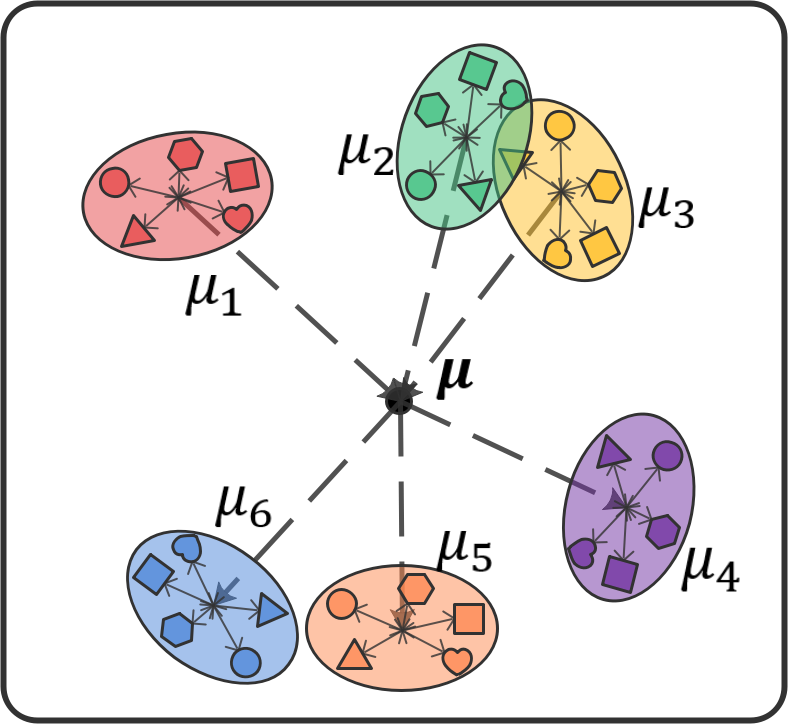
\includegraphics[width=0.95\linewidth]{figs/MvDA.png}
                \caption{MvDA}
            \end{subfigure}%
            \begin{subfigure}{0.15\textwidth}
                \centering
                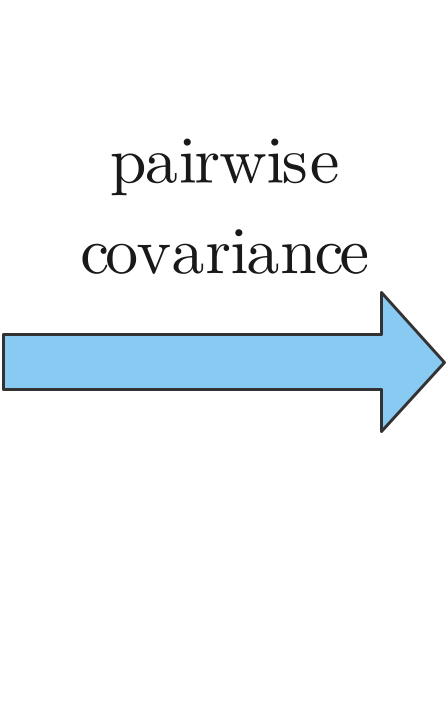
\includegraphics[width=1.0\linewidth]{figs/pc.png}
            \end{subfigure}%
            \begin{subfigure}{0.3\textwidth}
                \centering
                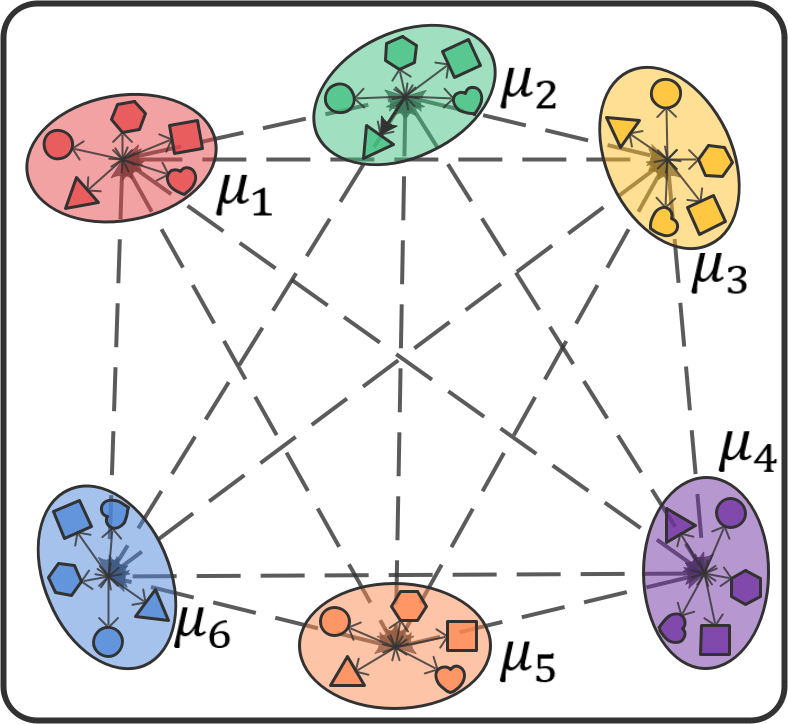
\includegraphics[width=0.95\linewidth]{figs/pc-MvDA.png}
                \caption{pc-MvDA}
            \end{subfigure}

            \caption{a) MvDA does not optimize the distance between paired classes in common space. b) pc-MvDA takes pairwise distances into account to better distinguish the classes.}
            \label{fig:pc-MvDA}
        \end{figure}

        Figure \ref{fig:synthetic1} shows MvDA and pc-MvDA results on 2D synthetic dataset of 180 data points in 2-D space.
        There are three classes (denoted by colors), observed at three viewpoints (denoted by shapes).
        This Figure displays original data distribution and 1-D projection results using MvDA and pc-MvDA respectively.
        Look closely, we can notice that data points of two classes (\textcolor{red}{red} and \textcolor{blue}{blue}) are well discriminated in each individual view but seems to have interchanged position in original space.
        In essence, $2^{nd}$ ($\bigtriangleup$) and $3^{rd}$ ($\square$) views share a similar layout while the $1^{st}$ ($\bigcirc$) view is flipped around the $y$ (vertical) axis.
        After projected in common space by MvDA, these classes are still close together as the common space constructed satisfies the criteria that distances between each class mean and global mean are maximized.
        In contrast, these classes are much more distinguishable when projected by pc-MvDA as it can find projections that undo the ``flipping'' in $1^{st}$ ($\bigcirc$) view to maximize pairwise distances.

        \begin{figure}[htbp]
            \centering
            \begin{subfigure}{0.33\textwidth}
                \centering
                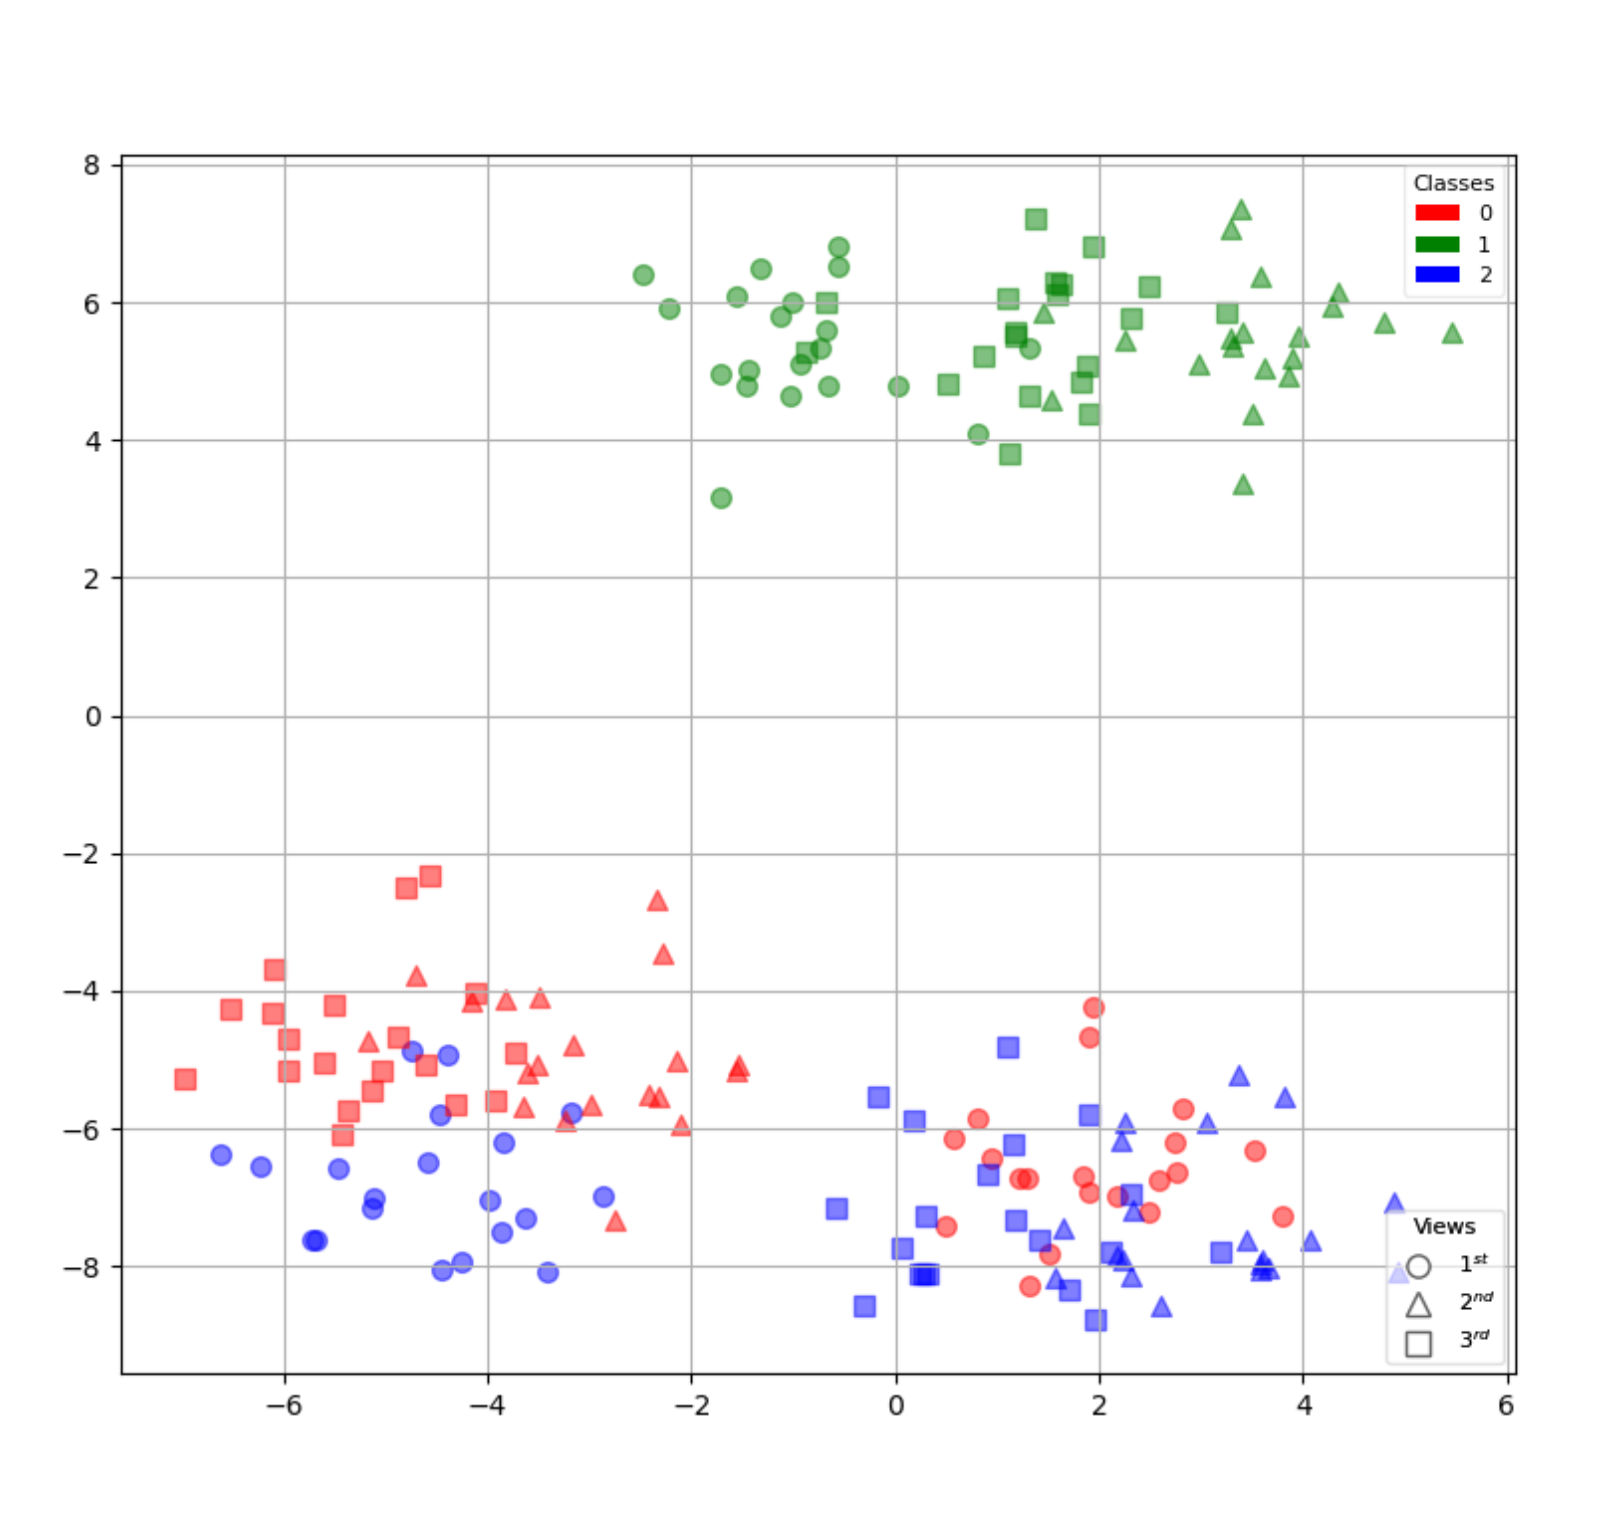
\includegraphics[width=0.95\linewidth]{figs/Synthetic1_original.png}
                \caption{Original distribution}
            \end{subfigure}%
            \begin{subfigure}{0.33\textwidth}
                \centering
                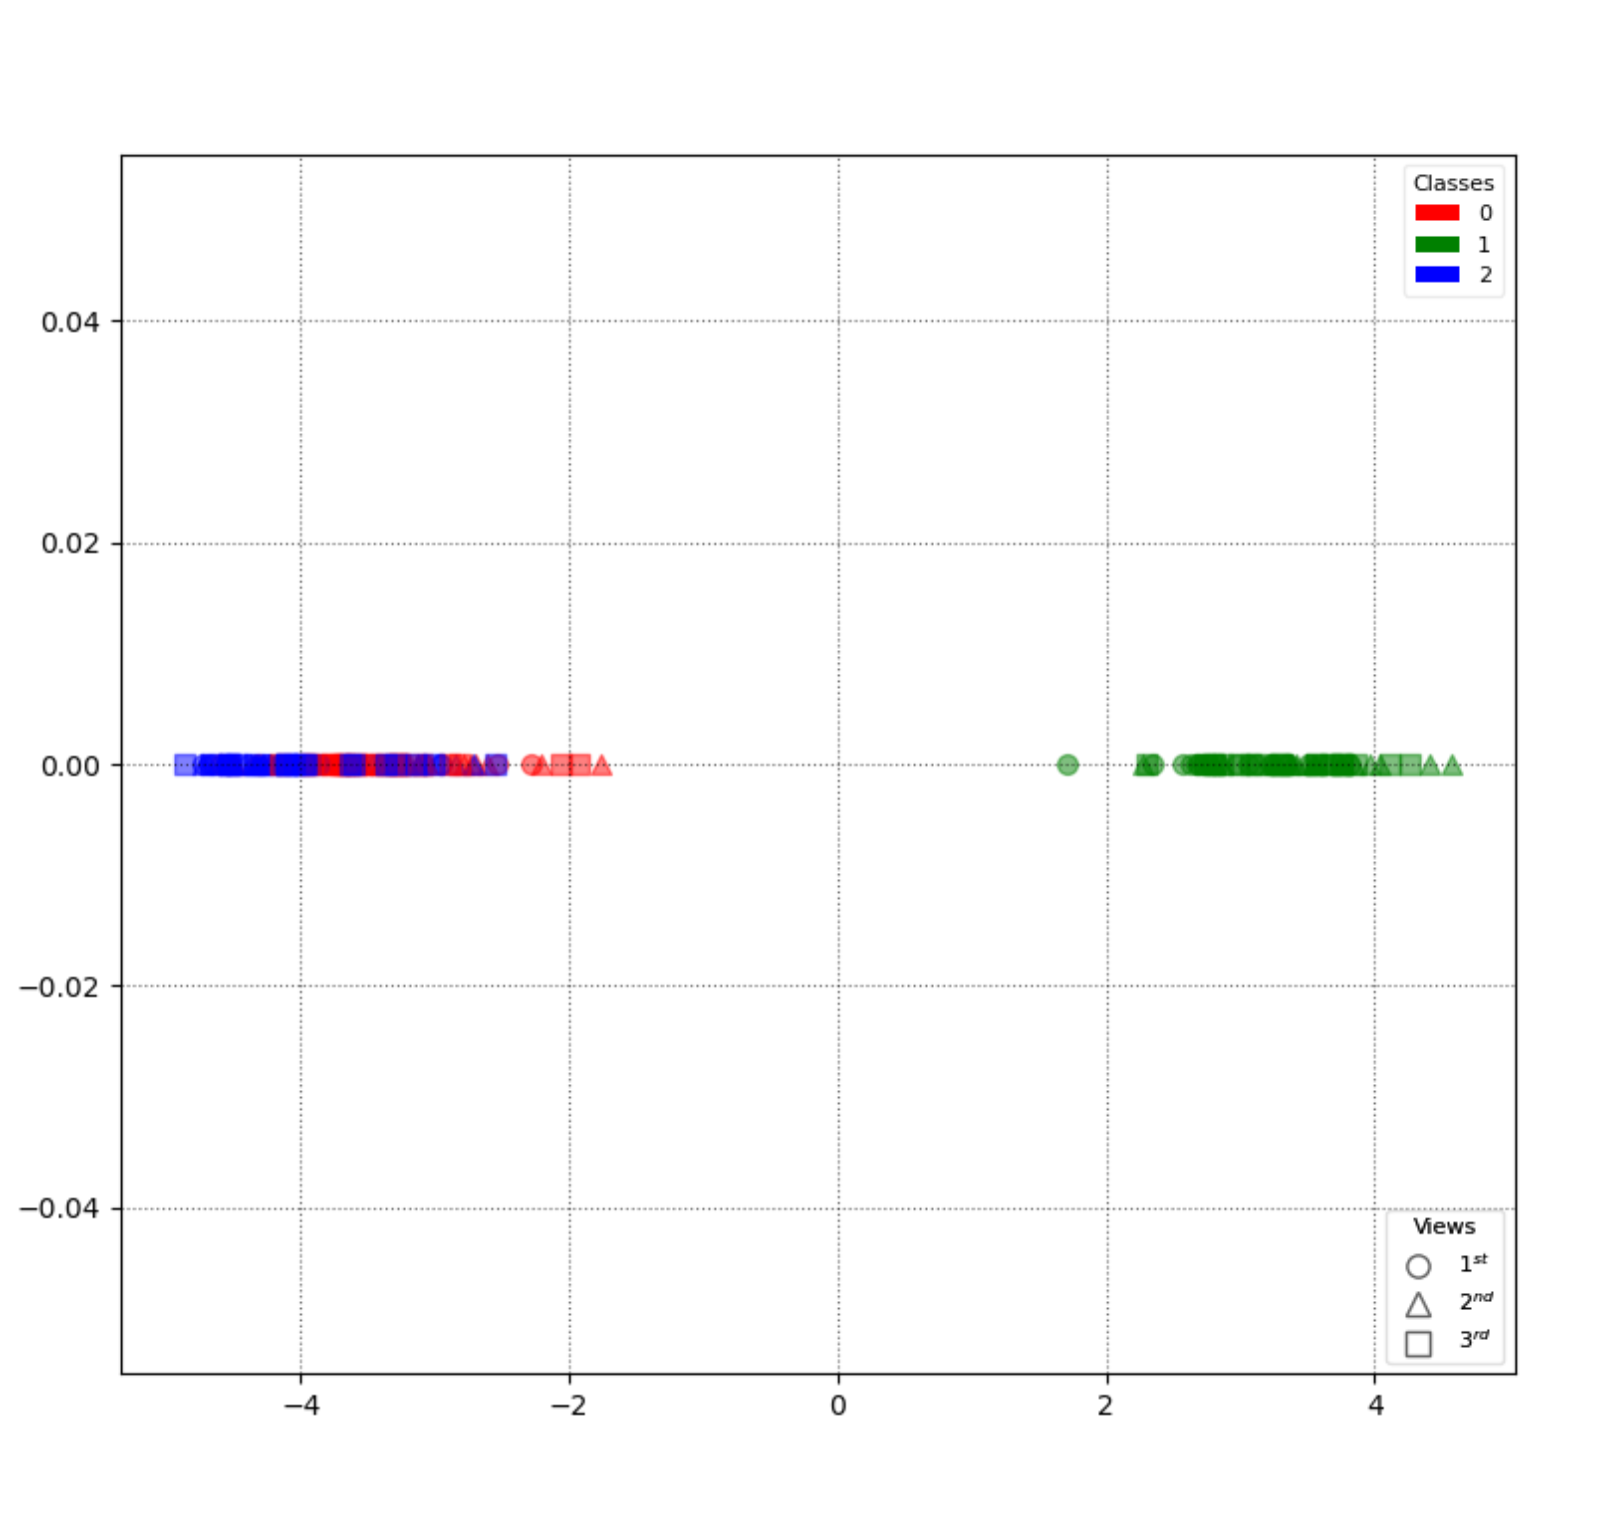
\includegraphics[width=0.95\linewidth]{figs/Synthetic1_MvDA.png}
                \caption{MvDA}
            \end{subfigure}%
            \begin{subfigure}{0.33\textwidth}
                \centering
                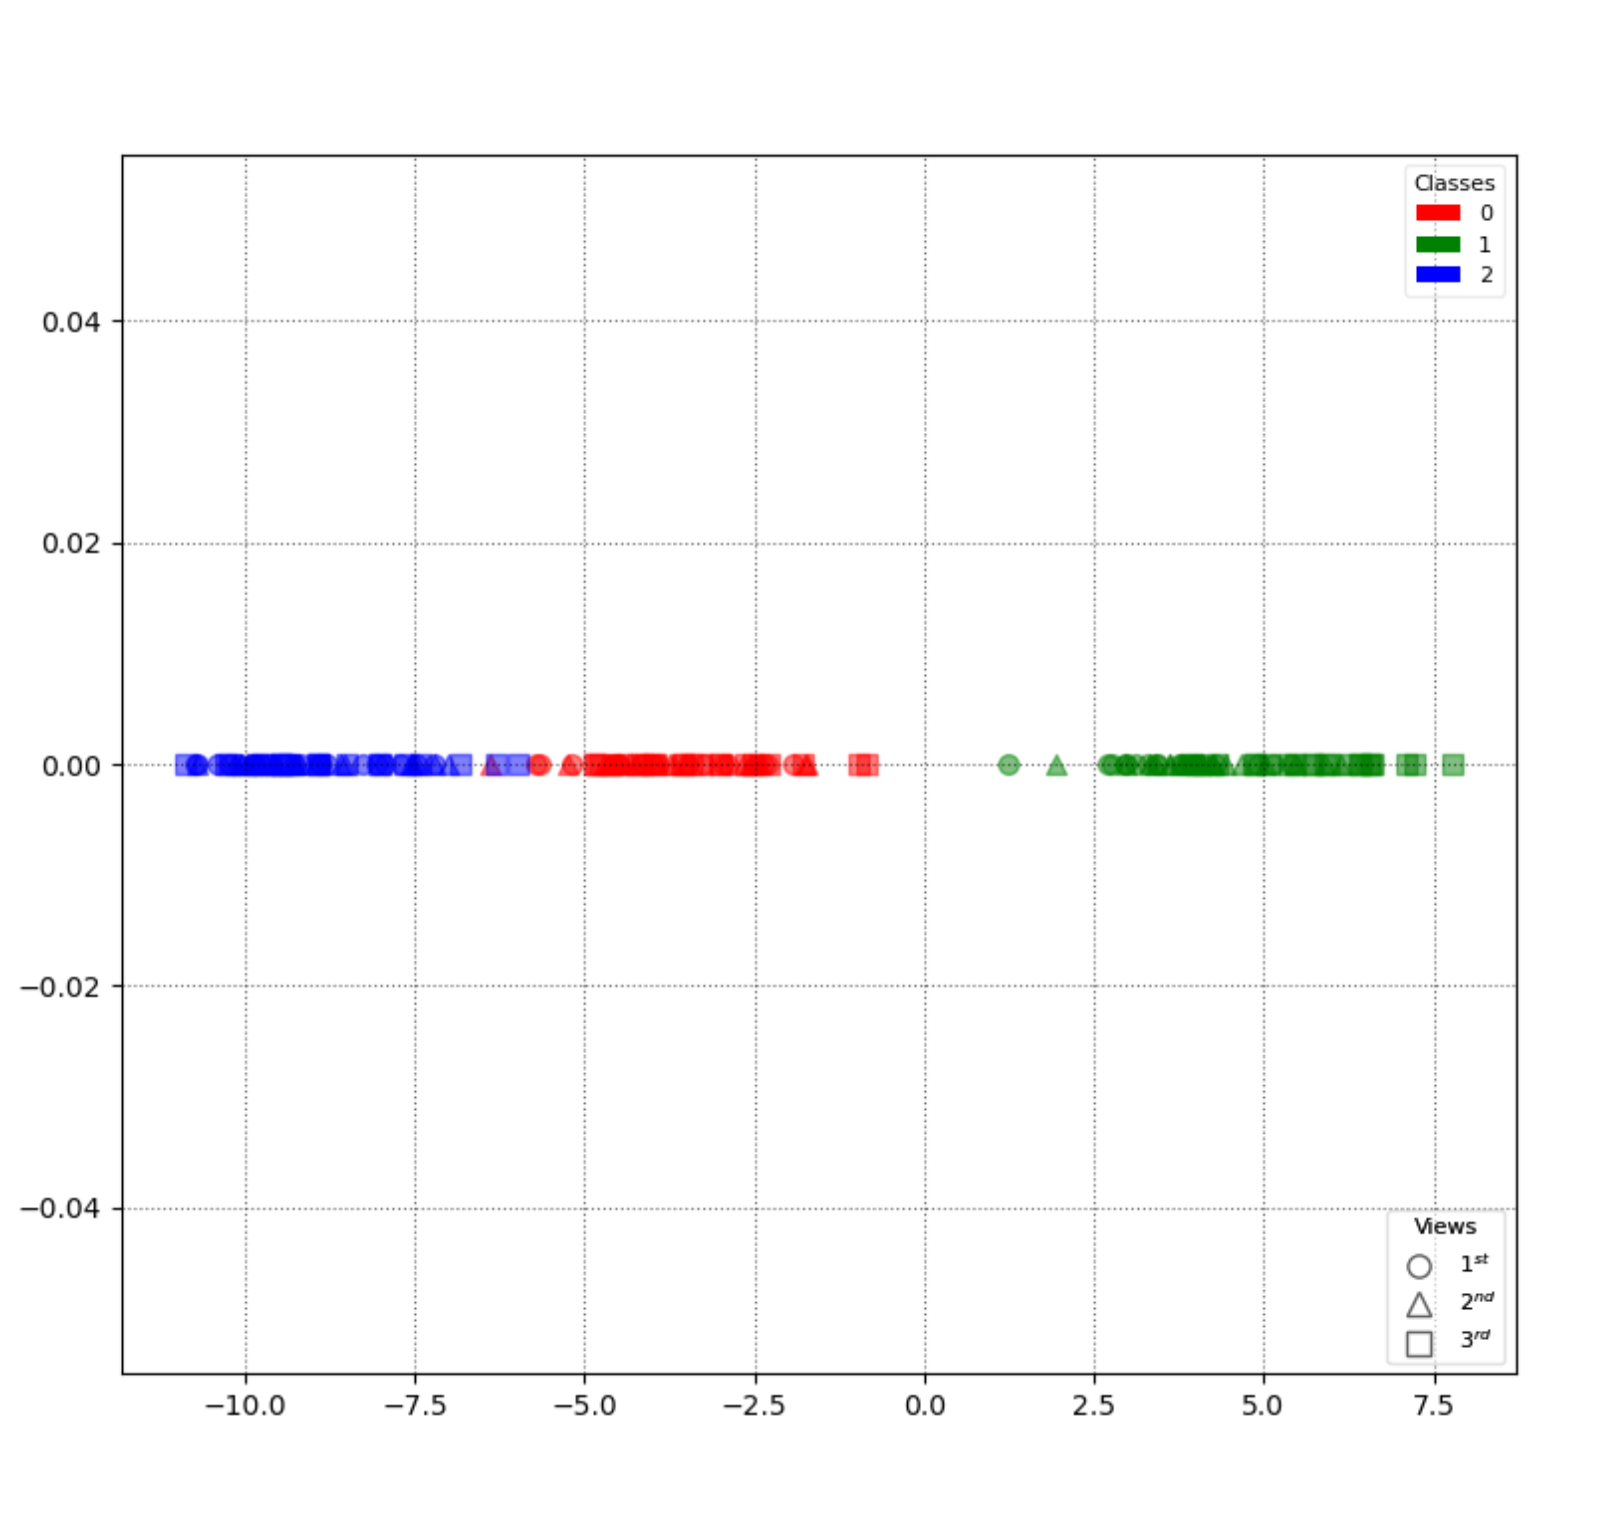
\includegraphics[width=0.95\linewidth]{figs/Synthetic1_pc-MvDA.png}
                \caption{pc-MvDA}
            \end{subfigure}

            \caption{A synthetic dataset of 180 data points, evenly distributed to 3 classes among 3 different views; a) 2-D original distribution; b) 1-D projection of MvDA; c) 1-D projection of pc-MvDA.}
            \label{fig:synthetic1}
        \end{figure}

        Similar to the first example, the second example consists of 300 data points of 5 classes observed from 3 different views (Figure \ref{fig:synthetic2}).
        We can observe that the five clusters of pc-MvDA common space contract strongly and become more separated as compared to the MvDA results (especially the \textcolor{red}{red} and \textcolor{yellow}{yellow} classes).
        The ablation study on synthetic datasets shows superiority of the proposed method.

        \begin{figure}[htbp]
            \centering
            \begin{subfigure}{0.33\textwidth}
                \centering
                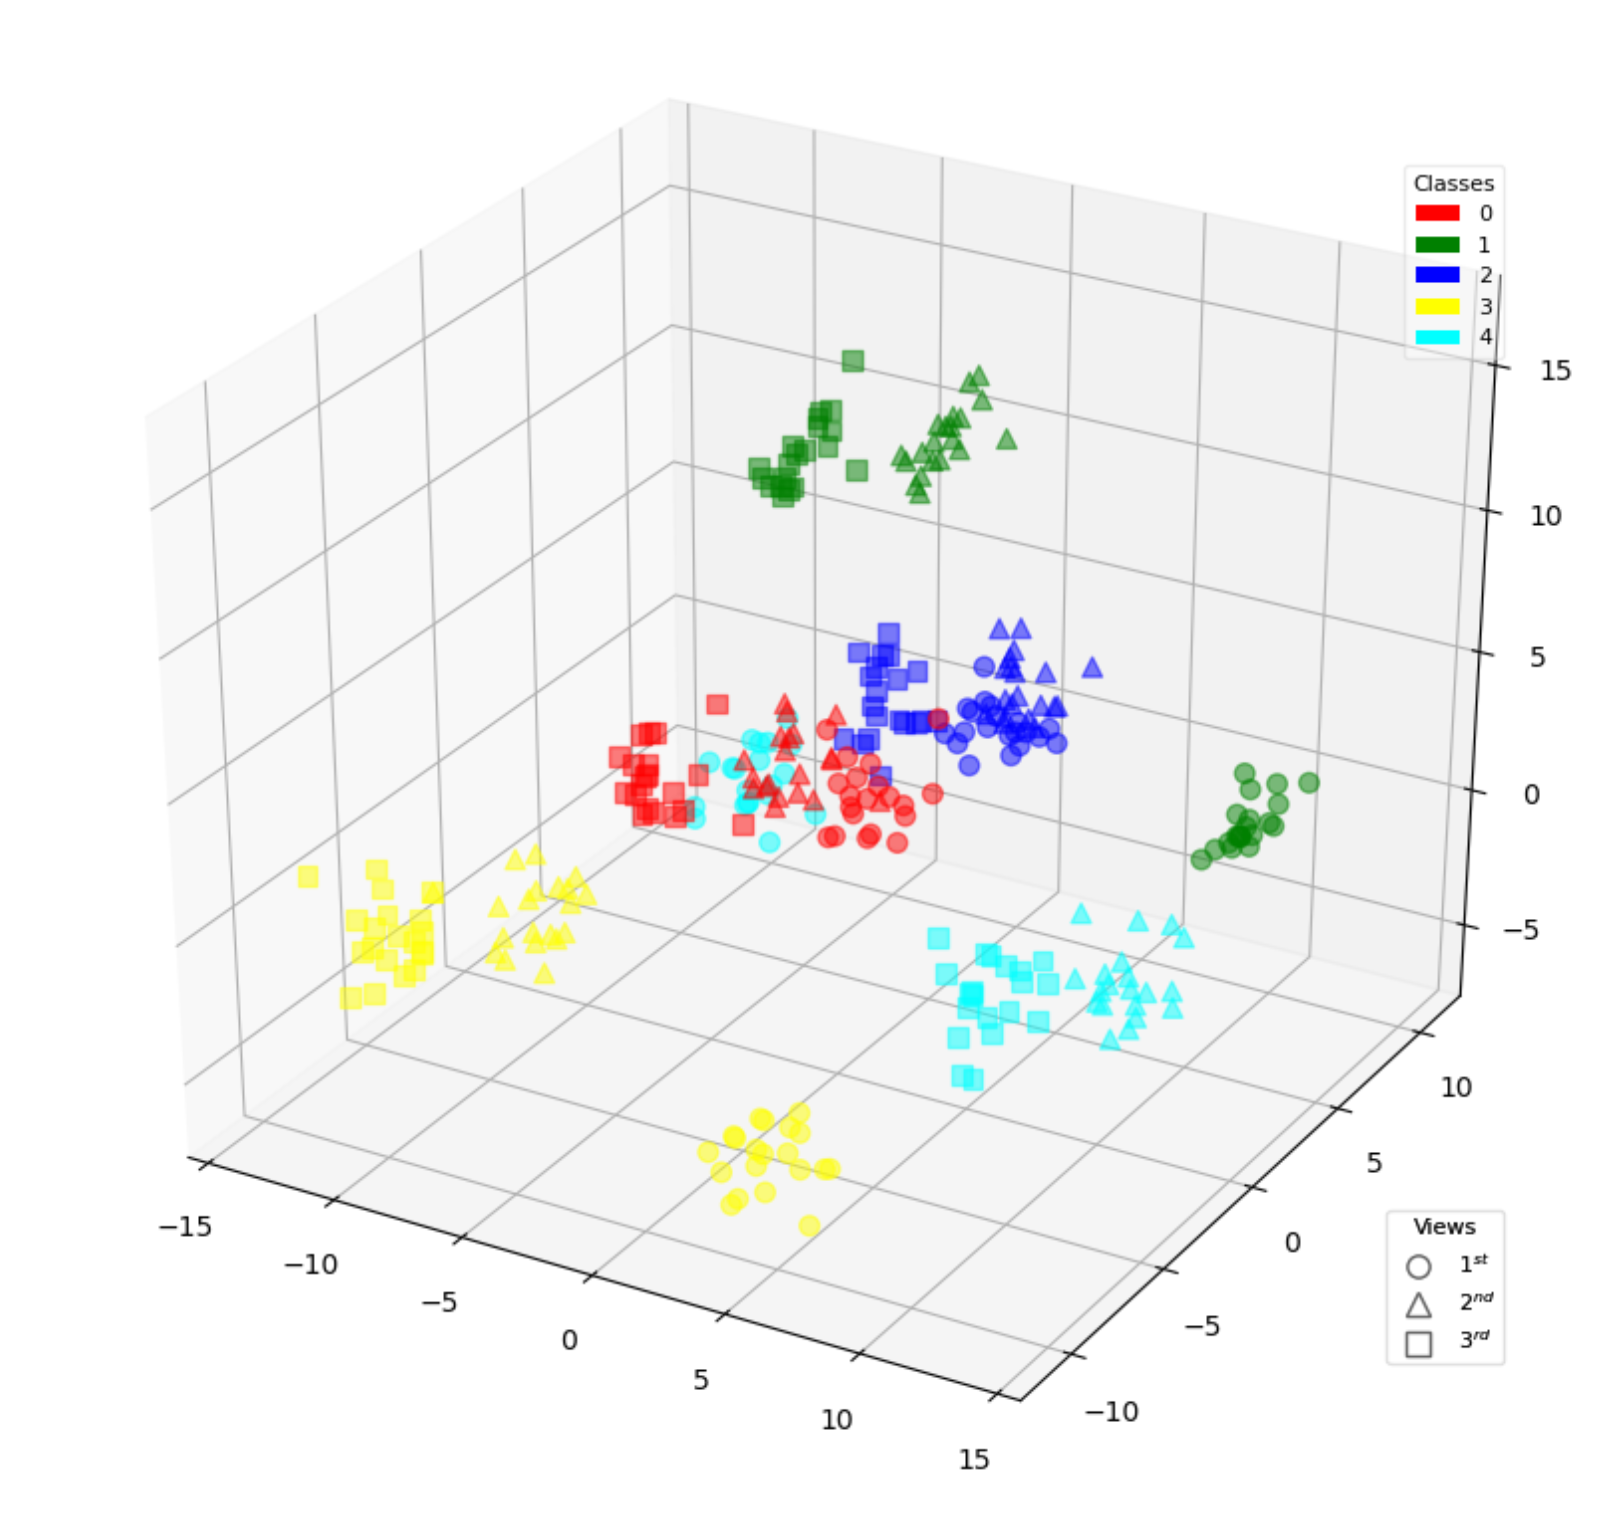
\includegraphics[width=0.95\linewidth]{figs/Synthetic2_original.png}
                \caption{Original distribution}
            \end{subfigure}%
            \begin{subfigure}{0.33\textwidth}
                \centering
                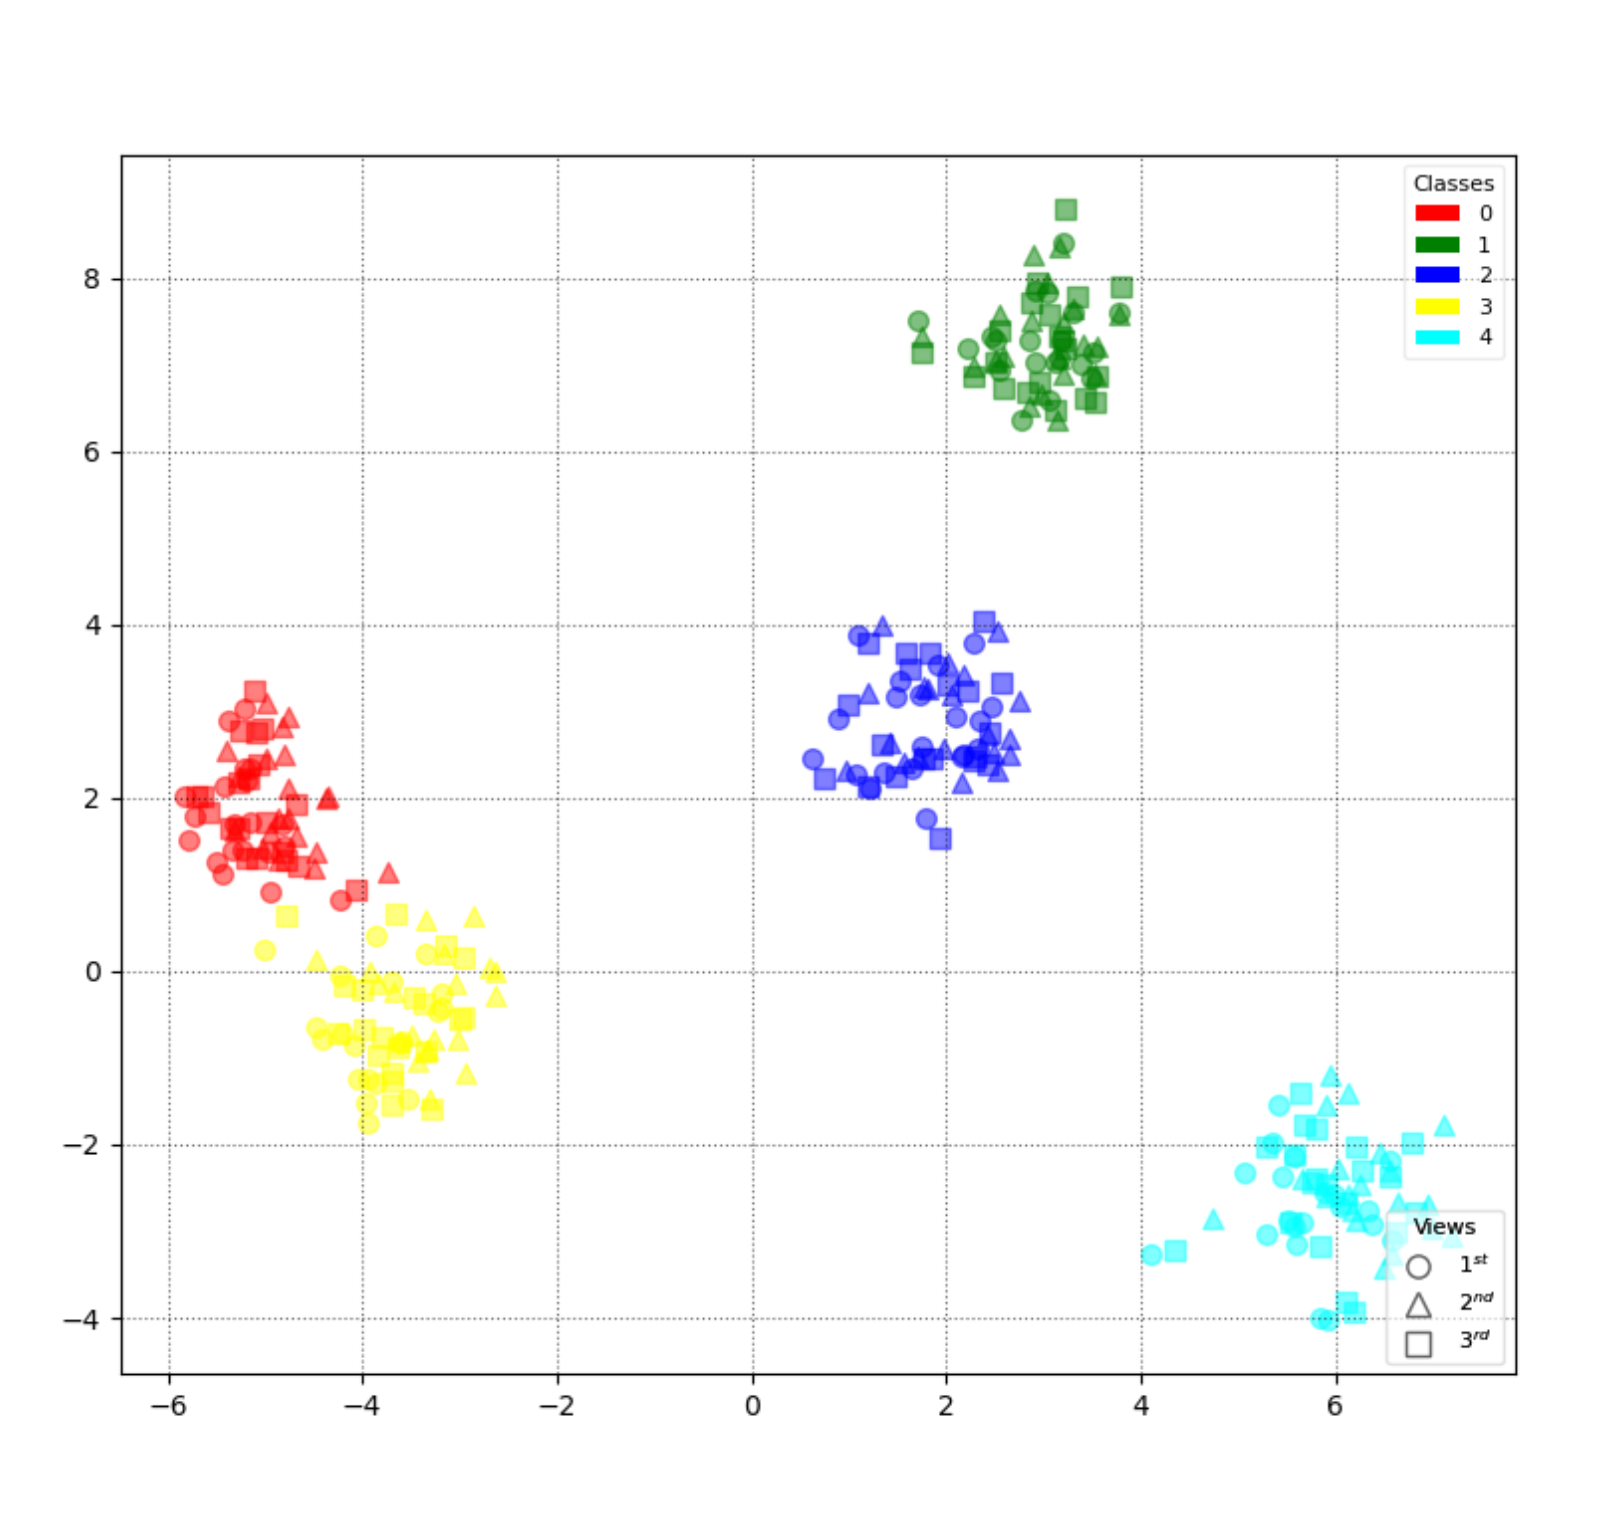
\includegraphics[width=0.95\linewidth]{figs/Synthetic2_MvDA.png}
                \caption{MvDA}
            \end{subfigure}%
            \begin{subfigure}{0.33\textwidth}
                \centering
                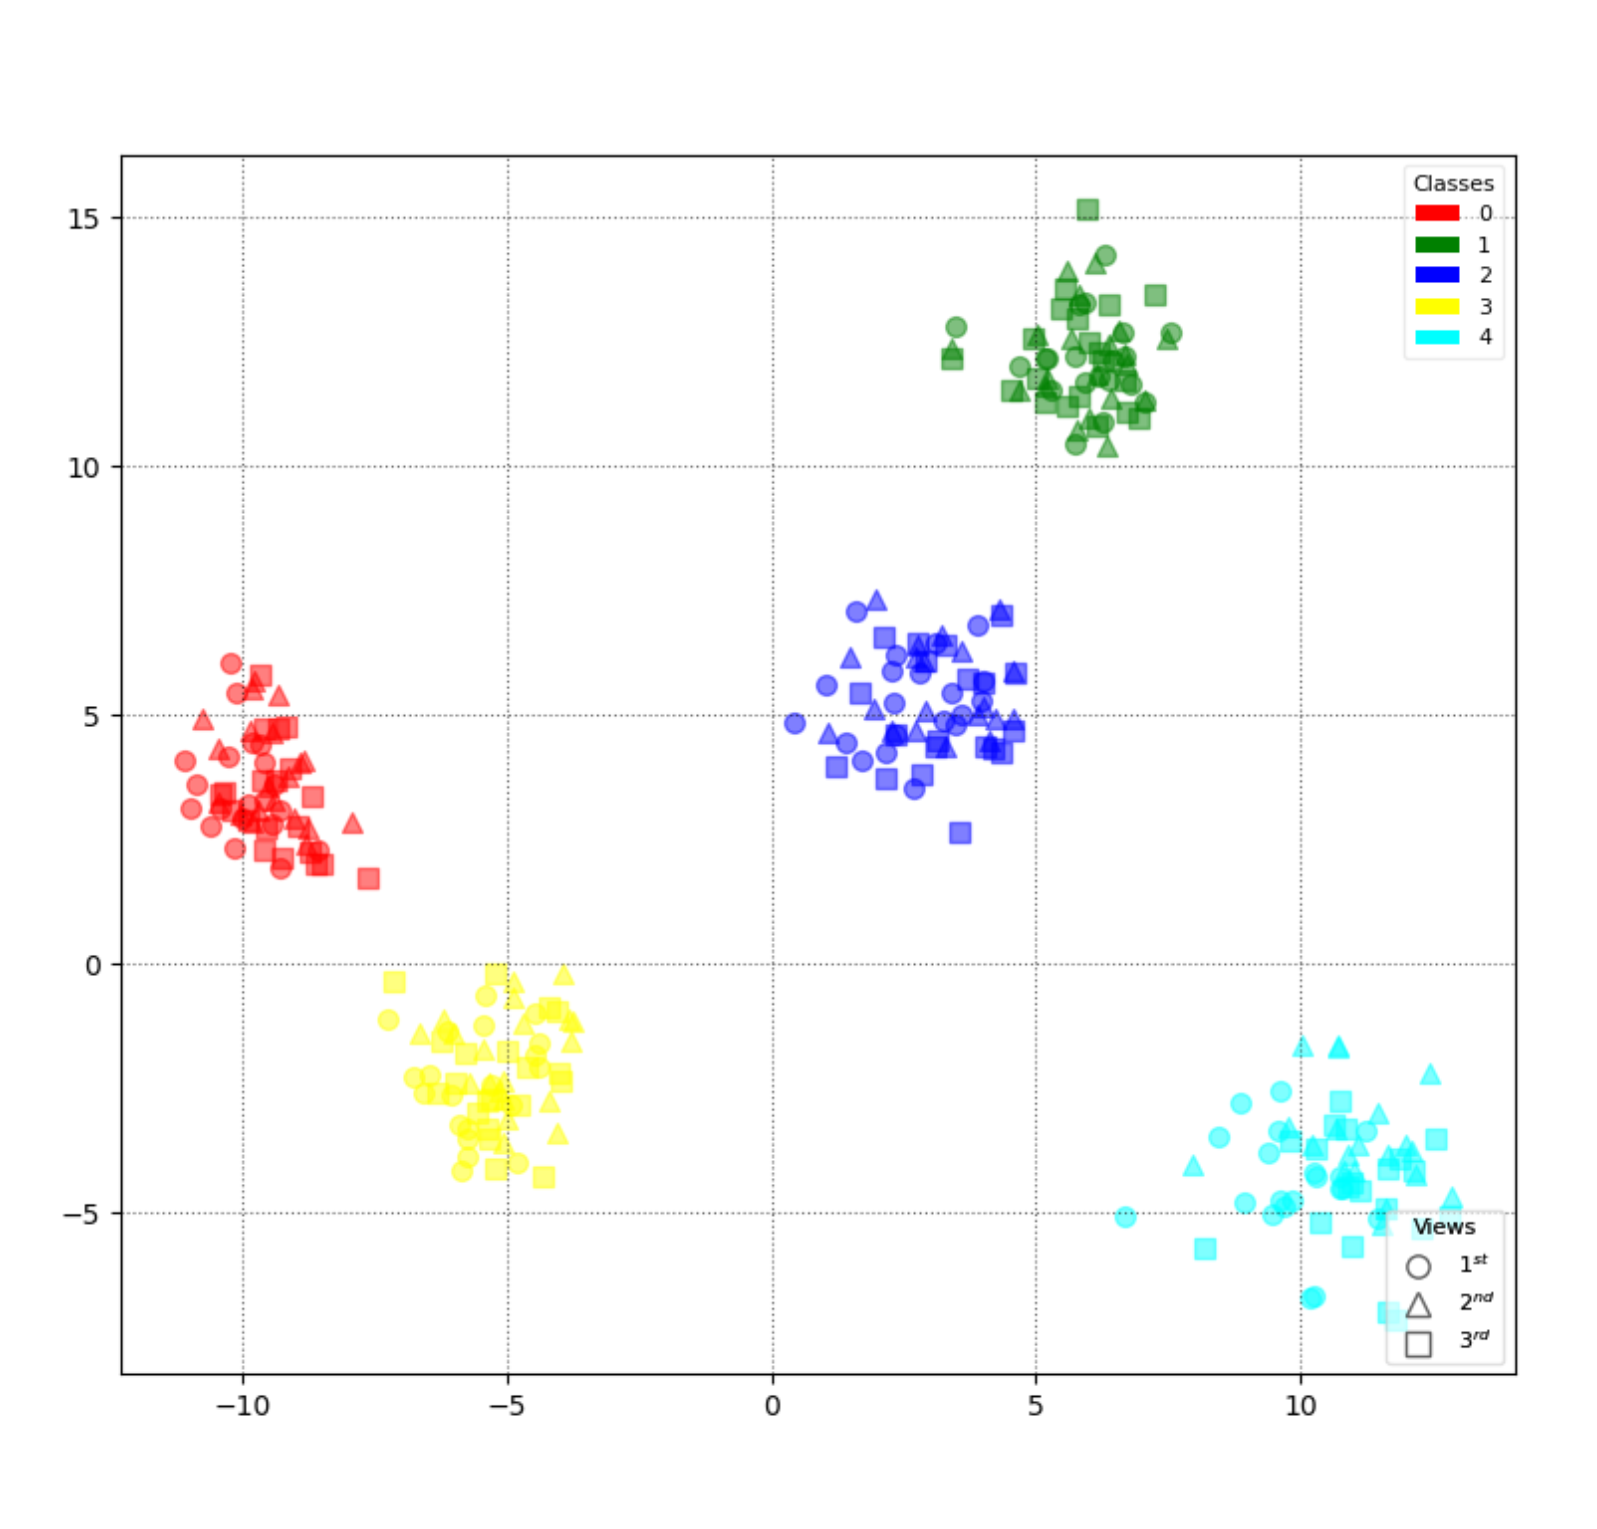
\includegraphics[width=0.95\linewidth]{figs/Synthetic2_pc-MvDA.png}
                \caption{pc-MvDA}
            \end{subfigure}

            \caption{A synthetic dataset of 300 data points, evenly distributed to 5 classes among 3 different views; a) 3-D original distribution; b) 2-D projection of MvDA; c) 2-D projection of pc-MvDA.}
            \label{fig:synthetic2}
        \end{figure}


    \paragraph{Algorithm to solve pc-MvDA}
        As the proposed objective does not match any optimization form of generalized eigenvalue problems, gradient descent algorithm is used to solve pc-MvDA. This approach also allow the algorithm to update incrementally even in higher dimensional data where the computation of matrix inversion and eigendecomposition are not conducive. The derivative of Equation \eqref{eq:pc-MvDA} is:

        \begin{equation}
            \frac{\partial J\left(W\right)}{\partial W}=-\sum_{a<b}^{c}{\frac{q n_a n_b}{n^2{J_{ab}\left(W\right)}^{q+1}}\frac{\partial J_{ab}\left(W\right)}{\partial W}}
        \end{equation}

        where $J_{ab}\left(W\right)=\sfrac{tr\left({\boldsymbol{S}_B^y}_{ab}\right)}{tr\left({\boldsymbol{S}_W^y}_{ab}\right)}$ is the Fisher loss of class pair $a$ and $b$. Its gradient is computed using the funky trace derivative and quotient rule:

        \begin{equation}
            \frac{\partial J_{ab}\left(W\right)}{\partial W}=\frac{tr\left({\boldsymbol{S}_W^y}_{ab}\right)W^T\left({\boldsymbol{S}_B^x}_{ab}+{{\boldsymbol{S}_B^x}_{ab}}^T\right)-tr\left({\boldsymbol{S}_B^y}_{ab}\right)W^T\left({\boldsymbol{S}_W^x}_{ab}+{{\boldsymbol{S}_W^x}_{ab}}^T\right)}{{tr\left({\boldsymbol{S}_W^y}_{ab}\right)}^2}
            \label{eq:grad_Jab}
        \end{equation}

        The superscript $x$ replacing $y$ in scatter matrices notations means that they denote the pre-transformed version. With simple algebra, we can rewrite the formulas in matrix multiplication form, separating transformation vectors $\omega_j$ in a concatenated matrix $W$ and a multi-view covariance matrix constructed from $v\times v$ cells, each cell $S^x_{jk}$ stands for the covariance between view $j$ and view $k$.

        \begin{equation}
            \boldsymbol{S}^y=W^T\boldsymbol{S}^xW=\left[\begin{matrix}\omega_1^T&\omega_2^T&\cdots&\omega_v^T\\\end{matrix}\right]\left[\begin{matrix}S^x_{11}&S^x_{12}&\cdots&S^x_{1v}\\S^x_{21}&S^x_{22}&\cdots&S^x_{2v}\\\vdots&\vdots&\ddots&\vdots\\S^x_{v1}&S^x_{v2}&\cdots&S^x_{vv}\\\end{matrix}\right]\left[\begin{matrix}\omega_1\\\omega_2\\\vdots\\\omega_v\\\end{matrix}\right]
        \end{equation}

        Specifically, ${\boldsymbol{S}^y_W}_{i}$ and ${\boldsymbol{S}^y_B}_{ab}$ from Equation \eqref{eq:pcmvda_Sw_i} and Equation \eqref{eq:pcmvda_Sb_ab} can be reformed as follows:

        \begin{align}
            {\boldsymbol{S}_W^y}_{i}  &= W^T {\boldsymbol{S}_W^x}_{i} W \ = W^T\left[X\left(\boldsymbol{I}_{i} - \boldsymbol{E}\right)X^T\right]W \label{eq:pcmvda_Sw_i_vec} \\
            {\boldsymbol{S}_B^y}_{ab} &= W^T {\boldsymbol{S}_B^x}_{ab} W = W^T\left[X\left(\boldsymbol{E}_{ab} - \boldsymbol{\tilde{E}}_{ab}\right)X^T\right]W \label{eq:pcmvda_Sb_ab_vec}
        \end{align}
        where $\boldsymbol{I}_{i}, \boldsymbol{E}_{ab}, \boldsymbol{\tilde{E}}_{ab} \in \mathbb{R}^{n\times n}$ are a square matrices whose definitions will be given in \nameref{chap:appendix}.

        Substitute \eqref{eq:pcmvda_Sw_i_vec} and \eqref{eq:mvda_Sw_vec} in Equation \eqref{eq:pcmvda_Sw_ab} we have:

        \begin{equation}
            \begin{split}
                {\boldsymbol{S}_W^y}_{ab} &= W^T{\boldsymbol{S}_W^x}_{ab}W \\
                &= W^T\left[X\left(\beta\left(\frac{n_a\boldsymbol{I}_a+n_b\boldsymbol{I}_b}{n_a+n_b}\right) + \left(1-\beta\right)\boldsymbol{I} - \boldsymbol{E}\right)X^T\right]W
            \end{split}
            \label{eq:pcmvda_Sw_ab_vec}
        \end{equation}

        The complete algorithm to compute $\nabla J$ is given in Algorithm \ref{algo:grad_computation}.

        \begin{algorithm}
            \SetKwInOut{Input}{Input}
            \SetKwInOut{Output}{Output}
            \SetEndCharOfAlgoLine{\relax}
            \Input{$W$, \{$X$, $\mu$\}, $q$}
            \Output{$\nabla J\left(W\right)$}
            $\boldsymbol{F} = 0$\;
            Compute $\boldsymbol{S}_W^x$ according to Equation \eqref{eq:mvda_Sw_vec}\;
            \For{$a=1$ \KwTo $c$} {
                \For{$b=a+1$ \KwTo $c$} {
                    Compute ${\boldsymbol{S}_B^x}_{ab}$ according to Equation \eqref{eq:pcmvda_Sb_ab_vec}\;
                    Compute ${\boldsymbol{S}_W^x}_{ab}$ according to Equation \eqref{eq:pcmvda_Sw_ab_vec}\;
                    Compute ${\boldsymbol{S}_B^y}_{ab}=W^T{\boldsymbol{S}_B^x}_{ab}W$\;
                    Compute ${\boldsymbol{S}_W^y}_{ab}=W^T{\boldsymbol{S}_W^x}_{ab}W$\;
                    Compute $J_{ab}=tr\left({\boldsymbol{S}_B^y}_{ab}\right)/tr\left({\boldsymbol{S}_W^y}_{ab}\right)$\;
                    Compute $\nabla J_{ab}$ according to Equation \eqref{eq:grad_Jab}\;
                    $\boldsymbol{F} = \boldsymbol{F} + n_an_b\nabla J_{ab}/J_{ab}^{(q+1)}$\;
                }
            }
            $\nabla J = {-q\boldsymbol{F}}/{n^2}$\;
            \Output{$\nabla J$}
            \caption{Computation of $\nabla J\left(W\right)$ (i.e. gradient of Equation \eqref{eq:pc-MvDA})}
            \label{algo:grad_computation}
        \end{algorithm}

        No further constraint is imposed to the proposed model. Although most modern programming frameworks do support the automatic deduction of $\nabla J\left(W\right)$ as backward process of computing the objective $J$, the above algorithm is derived for reimplementation in those that do not (i.e. Matlab).
        In fact, in my implementation of pc-MvDA in Pytorch, the computation of gradient is handled by automatic differentiation.
        % I choose Adam as optimizer with learning rate set to $0.01$.
        To have better starting point and mitigate variances, pc-MvDA is initialized with transformation learnt by MvDA.
